\section{Basic Architecture}
The core philosophy of Software-Defined Networking is horizontal disaggregation across every layers of the networking stack~\cite{systemsapproach}. Rather than relying on a vertically integrated, propriety hardware appliances, SDN decompose them into abstract components that is independent from other components, allowing each of which being used interchangeably and innovated at each layer.
\begin{itemize}
    \item \textbf{Local Network OS layer:} Physical switch hardware is decoupled from proprietary vendor software through bare-metal whitebox switches. Utilizing an Open Network Install Environment (ONIE) bootloader~\cite{onie}, the switch can load any compatible local Network OS (e.g., Stratum, SONiC) to handle local hardware initialization and peripheral management.
    \item \textbf{Control-to-Data Communication Interface:} The control plane and data plane interact over well-defined consumer/provider API endpoints using standard protocol (e.g. OpenFlow, gRPC/P4Runtime). This bidirectional interface allows controller to program forwarding rules while collecting real-time telemetry, link states, metrics, and packet from the data plane.
    \item \textbf{Device Driver \& Pipeline Layer:} This layer resolves hardware heterogeneity by splitting device control into low-level driver abstractions and pipeline-mapping logic. Analogous to a hardware SDK, the \textit{device driver} handles low-level chip management, translate control protocol messages (e.g., OpenFlow or P4Runtime) directly into chip memory while absorbing vendor-specific behavior mismatches. Sitting above the driver, the \textit{pipeliner} maps generic, high-level \textit{flow objectives} into the exact multi-table forwarding pipeline required by the underlying ASIC, freeing higher-layer application logic from needing to know the switch's internal table layout.
    \item \textbf{Data Plane layer: } Packet processing logic is completely decoupled from fixed-function hardware ASIC pipeline, allowing enterprise to implement custom header protocols on demand instead of waiting for switch vendor for the protocol implementation in their silicon chips. Using P4 language, packet parsing, header modifications, and forwarding behaviors can be programmed, updated, and recompiled directly on the hardware at runtime.
\end{itemize}
\subsection{Single-switch perspective: The Software Stack}
This includes an overview of a SDN stack with the involvement of a switch and controllers, highlight the top-to-bottom software stack being used in the SDN architecture. The main component include the Control App, Network OS, Switch OS, and P4 program--which used for the programmable switch. Figure 2 also introduced an exemplar of open-source software we used for this report (e.g. SD-Fabric, ONOS, Stratum), and protocol uses for communication between each layer.
\begin{figure}[H]
    \centering
    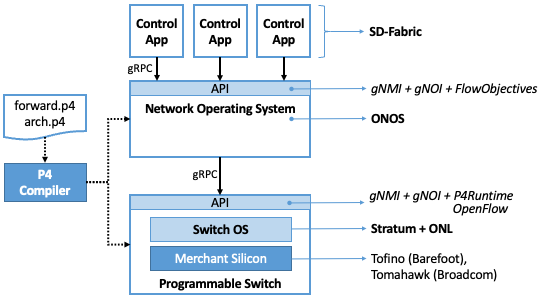
\includegraphics[width=1\linewidth]{graphics/image.png}
    \caption{Overall architecture of SDN stack with one switch. Adapted from \cite{systemsapproach}.}
    \label{fig:sdn-stack}
\end{figure}
At the top of the stack, Control Applications communicate with the Network OS via gRPC over Northbound APIs. Rather than writing raw table entries, applications issue high-level, topology-agnostic \textit{Intent}, or hardware-agnostic routing intents called \textit{Flow Objectives} (e.g., policy constraints or forwarding goals). Concurrently, management interfaces such as gNMI (gRPC Network Management Interface) and gNOI (gRPC Network Operations Interface) are exposed on the Northbound interface, enabling control applications to query dynamic network state (e.g., topology graphs, link statuses) and execute operational lifecycle commands (e.g., rebooting or upgrading devices).

Below the control abstraction is the separation of the control plane and the data plane. The Network OS compiles high-level Flow Objectives into low-level, device-specific \textit{Flow Rules}—concrete match-action entries targeted at explicit hardware table from the entire hardware pipeline. These rules are pushed down via gRPC using southbound protocols such as P4Runtime, OpenFlow, or gNMI. The local Switch OS (e.g., Stratum, originally developed by Google) receives these rules and programs the corresponding entries into the hardware switch silicon\footnote{Switch silicon refers to a specialized integrated circuit (ASIC) designed for line-rate packet processing, switching, and hardware-accelerated QoS management.}. Popular commercial implementations of this merchant silicon include Intel's Barefoot Tofino and Broadcom's Tomahawk chips.
\subsection{Network-Wide perspective: The Entire Network Data Path}
The previous subsection examined the SDN architecture through the lens of a single switch, a single controller, and its Network OS. This subsection zooms out to trace the data path end-to-end: from its origination at an end host, across one or more SDN-enabled switches, to its destination at another end host. As noted earlier, each switch along this path runs its own instance of a Switch OS, functioning as an on-host agent that programs flow rules onto the underlying silicon. The remainder of this subsection focuses on the end host itself, as the origination and termination point of the path; the inter-switch portion of the path---how multiple Switch OS instances are stitched together into a fabric under a common Network OS---is treated separately in Section~\ref{sec:onos} and the discussion of the Leaf-Spine Fabric.
\begin{figure}[H]
    \centering
    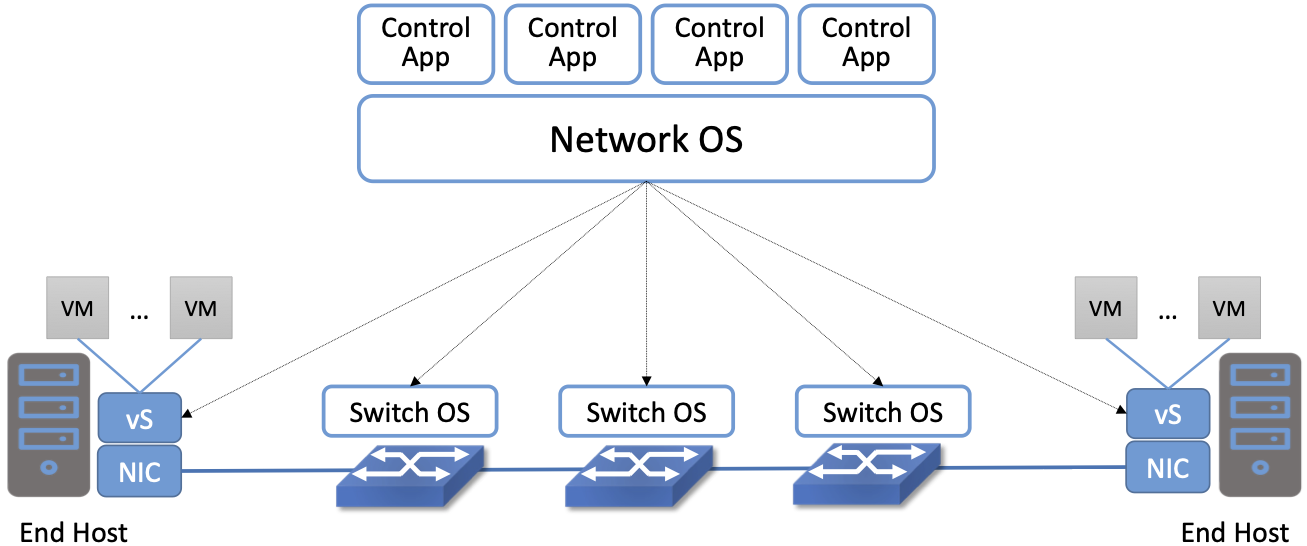
\includegraphics[width=1\linewidth]{graphics/network-wide sdn.png}
    \caption{End-End network view of SDN architecture. Adapted from \cite{systemsapproach}.}
    \label{fig:network-wide}
\end{figure}

With respect to the end host, Figure 3 highlights three components: the NIC, the virtual switch, and the VMs, all residing on the same physical server. A conventional NIC (Network Interface Card) is a hardware component that connects a computer or device to the network, converting data between the host's internal representation and the electrical or radio-frequency signals carried over the physical medium, and vice versa. The virtual switch (vSwitch, e.g., Open vSwitch) is a software switch that runs within the server's hypervisor and binds to the physical NIC as its uplink. Architecturally, the vSwitch occupies the same role as the Switch OS described in the single-switch view: it can be programmed by the same Network OS over southbound protocols such as OpenFlow or P4Runtime, receiving and installing Flow Rules exactly as a hardware Switch OS would. The distinction is one of substrate rather than function---the vSwitch executes its match-action pipeline in software on the host's general-purpose CPU~\cite{pfaff2015ovs}, whereas a physical switch executes the equivalent pipeline on dedicated ASIC silicon. Once programmed, it behaves as an ordinary switch, receiving packets on an input port and forwarding them to the appropriate output port; the endpoints attached to these virtual ports are typically Virtual Machines (VMs) or containers.

That said, this architecture rests on a few assumptions worth making explicit. First, not every end host runs VMs; the same picture applies to containerized or bare-metal hosts, with the vSwitch's virtual ports simply terminating at a different kind of endpoint. Second, the NIC--vSwitch--VM arrangement in Figure 3 is not the only valid way to structure the end host, but rather one particular perspective. This report, following~\cite{systemsapproach}, adopts a \textit{network-centric} view, in which the vSwitch and NIC are treated as an extension of the network, controlled by the same Network OS as the rest of the fabric. A \textit{host-centric} perspective is equally valid: it instead treats packet processing as a function of the host operating system itself, which means an architectural change in who is in control---instead of being managed by the network controller, it is configured directly by the host itself, via kernel-resident frameworks such as eBPF/XDP or user-space frameworks such as DPDK~\cite{systemsapproach}. Third, the conventional NIC introduced above is itself only one option: vendors have a long history of offloading kernel functionality onto the NIC, and this has led to the Smart Network Interface Card (SmartNIC), a NIC augmented with an FPGA or ASIC capable of running programmable logic. A SmartNIC can replace the conventional NIC, and, going further, can assist or even replace the vSwitch entirely by implementing part or all of its forwarding pipeline directly in NIC hardware~\cite{systemsapproach}. A more detailed treatment of these host-centric and SmartNIC-based alternatives, including their performance tradeoffs, is left for future work (Section~\ref{sec:research}), as it requires background this report has not yet developed.
